\documentclass[abstract=on,10pt,a4paper,bibliography=totocnumbered]{article}
\usepackage[paper=a4paper,left=35mm,right=35mm,top=25mm,bottom=30mm]{geometry}
\usepackage[doublespacing]{setspace}
\usepackage[english]{babel}
\usepackage[utf8]{inputenc}
\usepackage[round]{natbib}
\usepackage{amsmath}
\usepackage{colortbl}
\usepackage{amsfonts}
\usepackage{amssymb}
\usepackage{gensymb}
\usepackage{graphicx}
\usepackage{tikz}
\usepackage{enumerate}
\usepackage{enumitem}
\usepackage{subcaption}
\usepackage{booktabs}
\usepackage[hidelinks]{hyperref}
\usepackage[nameinlink]{cleveref}
% \usepackage{lineno}
\usepackage{multirow}
\usepackage{arydshln}
% \usepackage[nomarkers, nolists]{endfloat}

%------------------------------------------------------------------------------
%	Some Styling
%------------------------------------------------------------------------------
% Creating some TikZ styles
\tikzset{
  nonterminal/.style = {rectangle
    , minimum size = 6mm
    , very thick
    , draw = black!
  }
}

% Changing the style of captions in figures etc.
\captionsetup{labelfont=bf, format=plain, font=small}

% Change how equations are referenced
\renewcommand{\theequation}{Equation \arabic{equation}}%

%------------------------------------------------------------------------------
%	Titlepage: Header
%------------------------------------------------------------------------------
\title{Step by Step: Using Step Selection Analysis to Simulate Dispersal and
Assess Landscape Connectivity}

% List of Authors
\author{
  David D. Hofmann\textsuperscript{1,\S} \and
  John W. McNutt\textsuperscript{2} \and
  Arpat Ozgul\textsuperscript{1} \and
  Gabriele Cozzi\textsuperscript{1,2} \and
  Dominik M. Behr\textsuperscript{1,2}
}

% Reduce spacing between authors
\makeatletter
\def\and{%
  \end{tabular}%
  \hskip -0.5em \@plus.17fil\relax
  \begin{tabular}[t]{c}}
\makeatother

% Current Date
\date{\today}

% And here the masterpiece begins
\begin{document}

% Change page numbering
\pagenumbering{gobble}

% Required to be able to cite
\bibliographystyle{apalike}

% Create Titlepage
\maketitle

%------------------------------------------------------------------------------
%	Titlepage: Additional Info
%------------------------------------------------------------------------------
\begin{flushleft}

\vspace{0.5cm}

\textsuperscript{1} Department of Evolutionary Biology and Environmental
Studies, University of Zurich, Winterthurerstarsse 190, 8057 Zurich,
Switzerland.

\textsuperscript{2} Botswana Predator Conservation Trust, Private Bag 13, Maun,
Botswana.

\textsuperscript{\S} Corresponding author (david.hofmann2@uzh.ch)

\vspace{4cm}

\textbf{Running Title:} Release the Dogs! Simulating Wild Dog Dispersal to
Assess Landscape Connectivity

\vspace{0.5cm}

\textbf{Keywords:} dispersal, simulation, integrated step selection,
Kavango-Zambezi Transfrontier Conservation Area, landscape connectivity, Lycaon
pictus

\end{flushleft}

%------------------------------------------------------------------------------
%	Abstract
%------------------------------------------------------------------------------
\newpage
\begin{abstract}

During the past two decades, least-cost analysis and circuit theory have been
the two workhorses in connectivity analyses. This is largely thanks to their
ease of use and intuitive nature which has facilitated the application of the
methods across a broad range of animals. However, recent innovations in movement
ecology have brought forward new methods that are similarly intuitive but
provide several advantages over traditional connectivity modelling techniques.

Here, we propose the simulation of dispersal trajectories as a much more generic
way to identify dispersal barriers and potential movement corridors. Moreover,
we show how such simulations can be used to identify zones of high
human-wildlife conflicht, as well as to pinpoint potential "dispersal traps"
where dispersing individuals get trapped due to unavailability of suitable
alternatives. Finally, we discuss the benefits and pitfalls of dispersal
simualtions.
\end{abstract}

%------------------------------------------------------------------------------
%	Main Text
%------------------------------------------------------------------------------
\newpage

% Change page numbering
\pagenumbering{arabic}

% % Create linenumbers
% \linenumbers

\section{Introduction}
% Dispersal & Connectivity
Dispersal of individuals is an important process governing the dynamics wild
animal populations that are distributed in space \citep{Clobert.2012}. It is
defined as the movement of individuals from their natal location to the site of
first reproduction \cite{Howard.1960} and allows to avoid inbreeding
\citep{Perrin.1999, Perrin.2000, Frankham.2002, Leigh.2012}, to rescue small and
unviable populations \citep{Brown.1977}, and to promote the colonization of
unoccupied habitats \citep{Hanski.1998, MacArthur.2001}. Information on movement
behavior during dispersal and knowledge about the factors that limit dispersal
is therefore critical for a comprehensive understanding of landscape
connectivity and population viability \citep{Baguette.2013, Vasudev.2015}.

% Technological Advancements
Thanks to novel technologies developed over the past decades, particularly of
GPS/Satellite radio-collars, the study of dispersal has accelerated
\citep{Jonsson.2016, Williams.2019}. Additionally, the advent of publicly
accessible satellite imagery and sophisticated remote sensing techniques to
represent the physical landscape through which individuals disperse has pushed
the field towards a  ``golden age of animal tracking'' \citep{Kays.2015}.
Concurrently, the increased availability of large amounts of empirical data and
an increased computational power have led to the development of numerous
analytical methods to study movement behavior during dispersal
\citep{Boyce.2002, Fortin.2005, Cushman.2010, Zeller.2012, Elliot.2014,
Diniz.2019}.

% Measuring Connectivity
Resource selection functions \citep{Boyce.2002} and derived methods such as step
selection functions \citep{Fortin.2005} and path selection functions
\citep{Cushman.2010} have proven particularly useful for studying animal
movement and landscape connectivity. These methods allow estimating habitat
preferences of the focal species by comparing covariates at locations visited by
the animal to the scame covariates at locations available to, but not visited by
the animal. The so estimated preferences can then be used to predict a
permeability surface, indicating the expected ease at which an animal can
traverse a given area \citep{Zeller.2012}. Utimately, the permeability surface
serves as foundation to a connectivity model and to reveal movement corridors.
In this regard, the literature has long relied on least-cost methods
\citep{Adriaensen.2003} and circuit theory \citep{McRae.2006, McRae.2008}.
Unfortunately, both of these approaches make several limiting assumptions that
are hardly ever met in reality, particularly by dispersing animals. For
instance, to calculate a least-cost path one has to pre-define start- and
end-points. This implicitly assumes that animals have a preconceived end-point
in mind and choose a cost-minimizing route accordingly. To calculate a
least-costly route, one also needs to assume that animals have an infinite
perceptual range and that a route can always be realized, regardless of the
imposed costs. In contrast to least-cost methods, circuit theory assumes a
perceptual range of a single pixel, which is equally unrealistic and rarely
captures the scale of selection (cite someone). Moreover, directional biases
cannot be captured by circuit theory as a random walk is implicitly assumed. In
reality, however, dispersers often depict directional persistence and move in an
almost straight line to cover much ground very quickly. A mix of the two methods
can be seein in least-cost corridor approaches or randomized shortest paths have
been proposed to mitigate these issues by allowing animals to deviate from the
``optimal'' least-costly route \citep{Pinto.2009, Panzacchi.2016,
VanMoorter.2021}, they still fail to render a more realistic perceptual range of
the animal. In addition, neither of the two methods render the temporal
dimension of movement. Thusfar, only few have explored the usefulness of
individual based movement models when estimating landscape connectivity
\citep{Kanangaraj.2013, Hauenstein.2019, Zeller.2020}.

Nevertheless, collecting data on dispersers remains logistically challenging due
to dispersers' inherent mobility and due to the fact that dispersers only make
up a small fraction of the entire population, thereby making it difficult for
scientists to target apporpriate individuals for their study.

An animals movement trajectory can be seen as the result of an interplay between
habitat and movement preferences.

In recent decades, least-cost analysis has become the workhorse to study
landscape connectivty at large scales. Originally introduced by XX, the concept
and relating methods have been refined to more realistically render animal's
movement capabilities and to determine valuable movement corridors that require
protection. (talk a bit about different methods of LCPs, see methods in
gdistance package). More recently, more attention has been assigned to the
collection of movement data is better tailored towards assessing landscape
connectivity. In particular, it has been proposed and verified that relocation
data collected dispersing individuals leads to more accurate and reliable
estimates of landscape connectivity. This superiority of dispersal data in
comparison to data that stem from residents is mainly owed to the fact that
animals behave vastly different during residency. Despite substantial advances
in ecologists ability to track animals in space and time, dispersal remains one
of the most difficult behavioral modes to observe in wild animals. Especially
for wide ranging and long-lived species, dispersal is difficult to predict and
observe, such that data remains scarce.

Many connectivity modelling techniques, especially least-cost analysis,
implicitly assume that the studied animal has partial or even complete knowledge
of the landscape and associated movement costs. While this assumption may be
reasonable for migrating animals that move between a limited number of habitats,
yet it is unlikely to hold for dispersers. In contrast to migrants, dispersers
move into unknown territory and are therefore confronted with novel landscapes.
Consequently, dispersers are more likely to adjust their movement behavior
\textit{ad hoc} instead of preplanning an entire trajectory. As a result,
methods that assume complete knowledge of the landscape and subsequent optimal
movement behavior likely misrepresent true dispersal behavior. As such, methods
that allow a more random approach to a dispersers movement behavior may more
realistically render the movement corridors of dispersing individuals.

However, these models can not account for a correlation between turning angles
and step lengths, unless the two are sampled jointly from a copula distribution
(Hodel et al.).

A relatively recent addition to the step selection family has been integrated
step selection analysis.... Thanks to recently published papers and packages,
the suite of step selection functions has become accessible to most researchers
working with relocation data. Despite this, the use of such methods rarely
extends beyond assessing relative habitat preferences. However, once
parametrized, integrated step selection models could potentially serve as
powerful framework to simulate animal movement and assess landscape
connectivity. Here, we exemplify such analyses and show how ... coud be applied
to investigate ...

In contrast to Signer et et al, our focus lied on the transient utilisation of
the landscape.

In addition, individual based simulations will allow to explicitly model
dispersal between subpopulations in models of population dynamics.

Reliable identification of dispersal corridors will become increasingly
important with the uprise of ever-growing and often transboundary conservation
areas. One such instance is the KAZA-TFCA, a massive conservation area spanning
five countries and over 520'000 km\textsuperscript{2}. The KAZA holds the
potential of re-establishing dispersal routes for many of its protected species,
including the african wild dog \textit{Lycaon pictus}.  Persecution by humans,
habitat loss, and reduced connectivity are major causes of the decline of the
species \citep{Woodroffe.2012}. In result, the species currently marks the
KAZA's most endangered large carnivore and has been a assigned a very high
conservation priority. Importantly, due to their inherent mobility and intrinsic
need for vast undisturbed landscapes, AWDs have been proposed as surrogate
species for landscape connectivity (see recent paper on multispecies
connectivity). Nevertheless, the species has received little attention in the
connectivity literature, mainly due to the difficulty in observing wild dog
dispersal. In a previous paper, we addressed this issue and developed a habitat
selection model based on which we predicted landscape connectivity using
least-cost corridor analysis. We now expand on this knowledge and develop a more
detailed movement model of dispersing wild dogs. We then use this model to
simulate thousands of dispersers moving throughout the KAZA. Based on said
simulations, we compute heatmaps and identify potential dispersal hotspots and
compare them to the dispersal routes identified in (Hofmann ....). We also apply
the data to feed a network-analysis, based on which we determine network-metrics
pertinent to landscape connectivity.

\section{Methods}
\subsection{Study Area}
The study area (centered at -17\degree 13'9''S, 23\degree 56'4''E;
\Cref{StudyArea}a) stretched over 1.3 Mio km\textsuperscript{2} and ecompassed
the entire KAZA-TFCA (\Cref{StudyArea}b). The KAZA-TFCA is the world's largest
transboundary conservation area and comprises parts of Angola, Botswana,
Namibia, Zimbabwe, and Zambia, covering a total area of over 520'000
km\textsuperscript{2}. Its landscape varies regionally and ranges from savanna,
to grassland, and from dry to moist woodland habitats. A dominant
hydrogeographical feature in its center is the Okavango Delta, the earth's
largest inland delta. The delta and its surroundings are considered a stronghold
for African wild dogs and may act as a source for the recolonization of
surrounding habitats. The wet season within our study area lasts from November
to March and is out of phase with the main flooding of the Okavango Delta which
peaks between July and August \citep{McNutt.1996, Wolski.2017}.

\begin{figure}[htbp]
  \begin{center}
    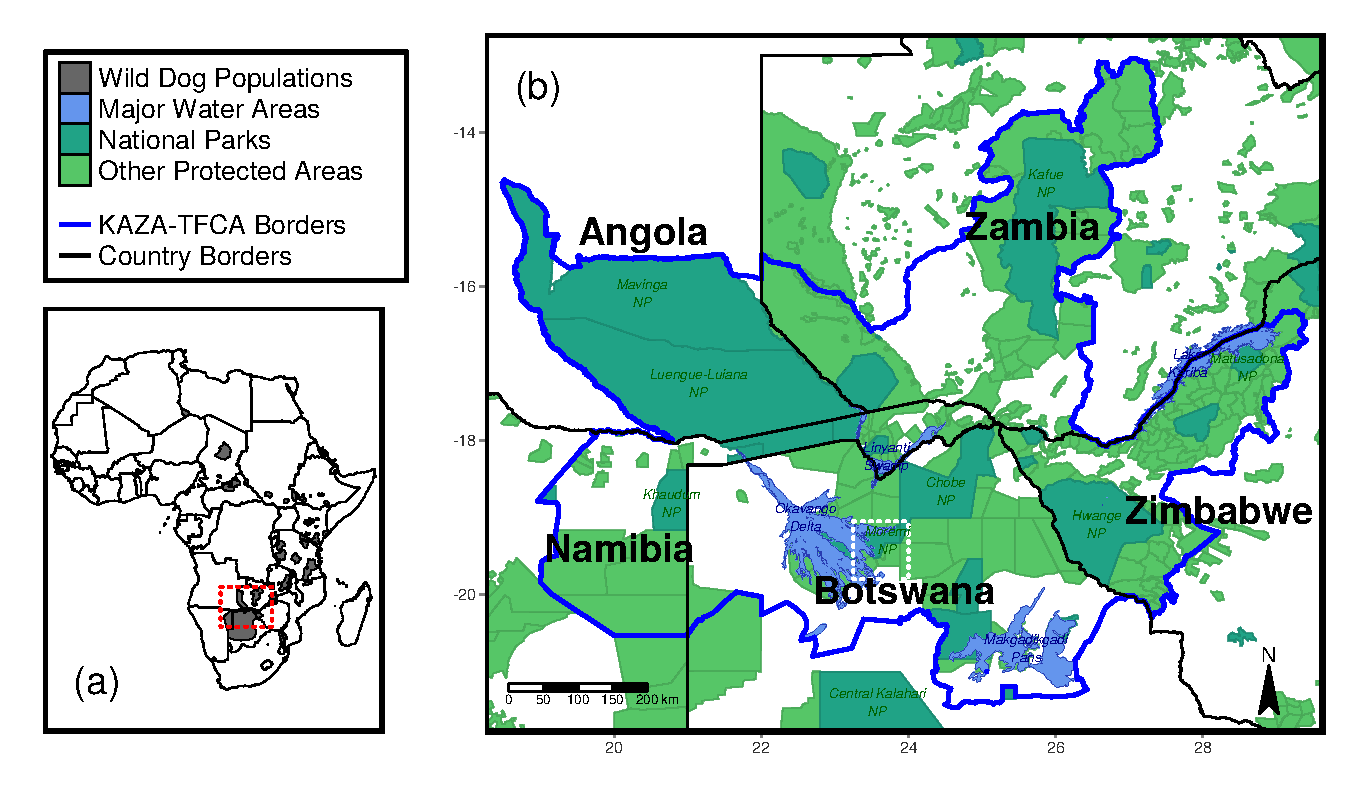
\includegraphics[width = \textwidth]{99_StudyArea.png}
    \caption{Study area}
    \label{StudyArea}
  \end{center}
\end{figure}

\subsection{GPS Relocation Data}
Between 2011 and 2020, we collected GPS relocation data on dispersing wild dogs
from a free-ranging wild dog population inhabiting the Okavango Delta in
northern Botswana. We identified potential dispersers based on age, number of
same‐sex siblings, pack size, and presence of unrelated individuals of the
opposite sex in their pack \citep{McNutt.1996, Behr.2020}. We immobilized
selected individuals using a cocktail of Ketamine/Xylazine/Atropine
\citep{Osofsky.1996, Cozzi.2020} which we injected with a dart, fired from a
CO\textsubscript{2}-pressurized gun (\textit{DAN-Inject, Denmark}). The
corresponding protocols have been approved by the Ministry of Environment,
Natural Resources Conservation and Tourism of Botswana (permit EWT 8/36/4
XXXVI). After immobilization, individuals were fitted with GPS/Satellite radio
collars (\textit{Vertex Lite; Vectronic Aerospace GmbH, Berlin}) that included
an automated drop-off mechanism. Handling and collaring of all individuals was
carried out and supervised by a Botswana-registered wildlife veterinarian. All
of the immobilized individuals quickly rejoined their pack after the procedure.
From all collared individuals, 16 individuals eventually dispersed in separate
same-sex coalitions and their trajectories were successfully recorded (7 female
and 9 male coalitions).

During dispersal, collars were programmed to record a GPS fix every 4 hours.
Recorded relocations were regularly transmitted over the Iridium satellite
system, which allowed remote tracking of individuals, even if they left the main
study area and crossed international borders. To effectively distinguish between
periods of residency and dispersal, we applied the net-squared displacement
metric to the observed movement data. This metric measures the squared Euclidean
distance of a collared individual to a reference point \citep{Borger.2012},
which we set at the center of each disperser's natal home range. Hence,
dispersal was deemed to have started when an individual left its natal home
range and ended when the individual became stationary again. For the purpose of
this study, we discarded andy data that was collected during residency. Because
previous research could not find any differences between males and females
during dispersal \citep{Woodroffe.2019, Cozzi.2020}, we did not distinguish
sexes for the sake of our analyses. Ultimately, we converted the collected GPS
relocations to steps, where a step represented the straight-line distance
travelled between two consequtive GPS relocations \citep{Turchin.1998}.

\subsection{Covariates}
To represent habitat covariates, we prepared a set of spatial raster layers
depicting water-cover (dynamically updated), distance to water (dynamically
updated), tree-cover, and shrub/grassland-cover. To render a decreasing impact
with increasing distance, we square rooted the distance to water covariate
layer. We also created a proxy for human influence, rendering anthropogenic
pressures stemming from human-density, agricultural sites, and roads. We
rendered all layers at a resolution of 250m by 250m for the entire extent of the
KAZA-TFCA. Further details on the derivation and preparation of each
environmental covariate is given in \cite{Hofmann.2020}.

Besides habitat covariates, we also computed movement metrics that we used as
movement covariates in our models. These covariates included the step length
(\(sl\)), its natural logarithm (\(log(sl)\)), as well as the cosine of the
relative turning angle (\(cos(ta)\)). Because wild dogs follow a diurnal
activity pattern, we furthermore coded a binary variable indicating whether an
observed step was realized during main activity (xx to xx) or low activity (xx
to xx).

\subsection{Movement Model}
We used integrated step selection functions (iSSF) to parametrize a mechanistic
movement model of dispersing wild dogs. In this framework, observed steps are
contrasted to random steps that the animal could have realized, but decided not
to. To compare steps, it is assumed that animals assign a relative selection
score \(w(x)\) to each step. The score depends on the covariates \(X\)
experienced along a step, as well as the animals preferences towards these
covariates \(\beta\). The probability of a step being realized is then
contingent on the step's selection score, as well as the selection scores of all
other step in the same stratum. In contrast to regular step selection analysis,
\textit{integrated} step selection analysis allows simulatneous inference on
movement and habitat preferences of the studied animal. Moreover, potential
interactions between habitat and movement preferences can be included to
investigate how movement behavior depends on habitat characteristics. In result,
the method produces less biased selection estimates and allows to apply the
resulting model as a fully mechanistic movement model based on which movement
can be simulated. To conduct iSSF analysis, we paired each observed step with 24
random steps. Random steps basically resembled potential alternatives that the
animal could have realized but decided not to. We generated random steps by
sampling random turning angles from a uniform distribution (\(-\pi, +\pi\)) and
step lengths from a gamma distirbution that was fitted to observed steps (scale
= 6'308, shape = 0.37). While the number of random steps is inversely
proportional to the sampling error \citep{Avgar.2016}, we found only minor
differences in model performance when sampling additional random steps and
deemed 24 random steps sufficient. Along each step, we extracted spatial
covariates using the \textit{velox} package and calculated the movement metrics
\(sl\), \(log(sl\)), and \(cos(ta)\). To facilitate model convergence, we
standardized all continuous covariates to a mean of zero and a standard
deviation of one. We then used the r-package \textit{glmmTMB} to fit mixed
effects conditional logistic regression models as proposed by \citep{Muff.2020}.

Our movement model was and extension of the habitat model presented in Hofmann
et al 2021. We will refer to it as the base model. Because the base model was
used to predict landscape permeability, no interactions between the habitat and
movement metrics were modeled. Thus, we expanded the base model and by proposing
additional interactions between movement metrics and environmental covariates.
For this, we started with the base model and iteratively increased model
complexity by adding all proposed two-way interactions between habitat
covariates and movement covariates. For instance, for the covariate
\textit{water} we proposed the interactions \(Water:log(sl)\),
\(Water:log(sl)\), and \(Water:cos(ta)\). Furthermore, we proposed the
interactions \(sl:cos(ta)\) and \(log(sl):cos(ta)\) to account for a correlation
between turning angles and step lengths, as well as the interactions
\(sl:MainActivity\) and \(log(sl):MainActivity\) to account for the fact that
step lengths diffuer due to the diurnal activity pattern. We then ran stepwise
model forward selection based on Akaike's Information Criterion (AIC,
\citealp{Burnham.2002}) values and identified the most parsimonious movement
model. Although several models received an AIC weight above one, we decided to
only consider the  ``best'' model for simplicity. In either way, the models with
positive weights contained almost identical covariates and an averaged model
would have only given weak support to additional covariates.

\subsection{Source Points}
We randomly placed source points within protected areas larger (\(>\) 700
km\textsuperscript{2}), which conforms to the average home range requirement of
resident wild dogs \citep{Pomilia.2015}. By distributing source points randomly,
the number of source points per km\textsuperscript{2} within protected areas was
approximately equal across our study area. In total, we distributed 50'000
source points across all protected areas, each representing the starting point
of a dispersal trajectory. To render potential immigrants into the study system,
we randomly placed 10'000 additional source points inside a xx km buffer around
the study area. Hence, a total of 60'000 source points were generated, thereby
resulting in 60'000 simulated dispersers. It is worth pointing out that our
choice of  placing source points completely random is arbitrary, as one as well
adjust the sampling frequency based on the density of dispersers in the
respective source area.

% Simulations from step selection functions are known to be sensitive to the
% location of source points, which is why we followed a twofold approach to sample
% release points across the KAZA-TFCA. In a first approach, we used the same 68
% source points between which we already computed least-cost paths and least-cost
% corridors (see xx). These source points were regularly spaced 100 km apart,
% located within protected areas (\(>\) 700 km\textsuperscript{2}). Because of
% the regulary spacing, not all protected areas received source points. Hence, we
% placed additional source points at the center of such protected areas. At each
% of the generated source point we released 1000 dispersers, implying a total of
% 68'000 simulated dispersers. In a second approach, we used the same 68 source
% points to define catchment areas inside protected areas. That is, for each of
% the 68 source points we defined its voronoi polygon within the point's protected
% area. Within these catchment areas we then randomly sampled 1000 new source
% points from which we released another 68'000 dispersers. Overall, we simulated
% 134'000 dispersers for a total of 268 Mio. steps.

\begin{figure}[htbp]
  \begin{center}
    \includegraphics[width = \textwidth]{99_SourcePoints.png}
    \caption{Illustration of source points from which dispersal was simulated.
    Although in reality we simulated 1'000 per source point, we illustrate an
    example assuming 10 dispersers from each source point. (a) Static source
    points similar to the source points reported in ... (b) Source points that
    were randomized within the catchment areas (dark gray, delinated by solid
    black lines).}
    \label{SourcePoints}
  \end{center}
\end{figure}

\subsection{Dispersal Simulation}
We used the most parsimonious movement model to simulate dispersing wild dogs
departing from the above described source points. The simulation resembled an
inverted iSSF and was set up as follows. First, we determined a source point at
which a disperser was initiated. To allow calculation of turning angles, we
assumed a random orientation of the animal. Second, we proposed a set of 25
random steps leaving from the source point. We generated random steps by
sampling turning angles from a uniform distribution (\(-\pi, +\pi\)) and step
lengths from our fitted gamma distribution. To prevent unrealistically large
steps, we capped sampled step lengths at 35km, which is the farthest distance
travelled by our dispersers within 4 hours. Third, along each random step we
extracted habitat covariates and calculated movement covariates. Fourth, we
applied the parametrized movement model to predict the selection scores \(w(x)\)
for all steps. Fifth, we translated selection scores into probabilitities by
applying equation xy. Sixth, we sampled one of the proposed based on assigned
probabilities and calculated the animal's new position. We then repeated steps
two to six until a total of 2000 steps were realized.

To mitigate the influence of edge effects, we added a buffer zone around each
covariate layer. The values within the buffer zone where resampled from the true
data. As such, simulated dispersers were allowed to leave and reenter the study
area through this buffer zone. In case one of the proposed random steps left the
outer boundary of the buffer, we replaced the step with an alternative step that
lied fully within the buffer zone. Thus, we force the disperser to bounce of the
borders of the study area.

\subsection{Heatmaps}
Using the simulated trajectories, we created heatmaps that indicate the
frequency at which each raster-cell in the study area was visited. If the same
trajectory crossed a pixel twice, it was only counted once, i.e. we did not
consider revisits. We achieved high performance rasterization of all simulated
trajectories using the recently developed R-package \textit{terra}
\citep{Hijmans.2020}.


To examine if and how ``heat'' changes in response to changes in the location of
source points and the number of simulated steps, we followed a 2 x 6 design and
created heatmaps for both point sampling regines, as well as for 68, 125, 250,
500, 1000, and 2000 dispersal steps. We quantified the similarity of the
resulting 12 heatmaps to the permeability and least-cost corridor maps presented
in (Hofmann ...) we used Bhattacharyya's affinity. Bhattacharyya's affinity
ranges from zero (complete separation) to one (perfect match) and has earlier
been proposed to compare the overlap of utilisation distributions (Fieberg).


\subsection{Betweenness}


\subsection{Network Analysis I: Areas Reached}
Based on the simulated trajectories we identified to which other areas each
source area is connected. For instance, if a trajectory originated at source
point one and intersected with source areas two and three, we assumed that
source areas two and three were within reach of source are one. To get a sense
of the strength of connections, we also calculated how often each of these
connections was realized. This procedure resulted in 6 x 2 edge lists which we
further used to generate weighted networks and to calculate network metrics.

\subsection{Network Analysis II: Betweenness}
We coerced all simulated trajectories into a network consisting of vertices
(relocations) and edges (connections between relocations). To do so, we created
raster layers at multiple resolutions and identified each trajectory's
transition matrix on these rasters see figure xx \citep{BastilleRousseau.2018}.
We then merged the transition matrices of all trajectories and calculated
cumulative transitions between all raster-cells. This resulted in an edge-list,
containing all observed from-to connections as well as their frequency. Using
this edge-list, we generated a weighted graph using the r-package
\textit{igraph}. Based on this graph we calculated betweenness scores as well as
the degree of each raster cell. Betweenness indicates how often a specific
raster-cell lies on a shortest path between two other raster-cells and is a
useful metric to detect movement corridors. Degree, on the other hand, indicates
how many connections a raster cell has and therefore serves to illustrate the
xxx of specific nodes. When calculating betweenness, we used the transition
frequency as weighting factor. That is, a higher transition frequency
contributed to a higher betweenness score.

\subsection{Network Analysis III: Transitions}



\section{Results}
Compared to the base model, the most parsimonious movement model included
several additional interactions (\Cref{MovementModel} and Table S1). The model
indicates that dispersers move directional, particularly when distant to water,
yet less so in human dominated landscapes. Furthermore, dispersers prefer large
steps, especially during main activity. In contrast, step lengths tend to be
shorter when water- or tree-cover is high. In general, dispersers avoid water,
prefer proximity to water, avoid dense tree-cover, prefer shrubs/grassland, and,
finally, avoid human dominated landscapes.

\begin{figure}
  \begin{center}
    \includegraphics[width=\textwidth]{99_MovementModel}
    \caption{(a) Most parsimonious movement model for dispersing wild dogs. The
    model includes a habitat kernel, a movement kernel, as well as their
    interactions. The orange and blue line segments delineate the 90\%, 95\%,
    and 99\% Confidence-Intervals around the respective \(\beta\) coefficients.
    Significance codes: * \(p < 0.10\), ** \(p < 0.05\), *** \(p < 0.01\). (b)
    Results from the k-fold cross validation procedure. The upper plot shows
    rank frequencies of predicted realized scroes according to model predictions
    with known preferences, whereas the lower plot shows rank frequencies when
    assuming random preferences. The blue ribbon shows the prediction interval
    around a loess smoothing regression that we fitted to ease the
    interpretation of the plots.}
    \label{MovementModel}
  \end{center}
\end{figure}

\subsection{Heatmaps}
Six of the twelve rasterized dispersal trajectories are presented as heatmaps in
\Cref{Heatmaps}. As can be seen, differences that stem from the method of point
sampling disappear as more steps are simulated. This is to be expected as the
influence of the origin becomes smaller and smaller as the animal moves through
the landscape. However, there are striking differences when simualtions are only
run for few iterations.

\begin{figure}
  \includegraphics[width=\textwidth]{99_Heatmaps}
  \caption{}
  \label{Heatmaps}
\end{figure}

Bhattacharyya's affinity index supports the notion that heatmaps become more
similar to the earlier developed permeability and corridor maps as the number of
simulated steps increases. Furthermore, it appears that randomly sampled source
points contribute to a higher similarity too, albeit differences due to the
sampling regime vanish as the number of simulated steps increases. In fact, both
maps are almost identical to each other after 2000 steps. Furthermore, the
connectivity networks become increasingly similar to the previously published
permeability and corridor maps. Still, some differences remain even after 2000
simulated steps, highlighting that some severe impediments in the landscape
exist.

\begin{table}[hbtp]
  \caption{Summary statistics of all GPS relocations that have been recorded on
  dispersing coalitions.}
  \label{GPSData}
  \begin{center}
  \resizebox{\textwidth}{!}{
    \begin{tabular}{lllllllll}
    \toprule
    sampling & Metric & Map & 68 & 125 & 250 & 500 & 1000 & 2000 \\
    \midrule
    Static & Affinity & Corr & 0.64 & 0.70 & 0.76 & 0.80 & 0.82 & 0.84 \\
    Static & Affinity & Perm & 0.67 & 0.74 & 0.80 & 0.85 & 0.89 & 0.91 \\
    Static & Correlation & Corr & 0.32 & 0.38 & 0.45 & 0.51 & 0.56 & 0.60 \\
    Static & Correlation & Perm & 0.47 & 0.57 & 0.66 & 0.72 & 0.78 & 0.82 \\
    \hdashline
    Random & Affinity & Corr & 0.70 & 0.75 & 0.79 & 0.82 & 0.84 & 0.85 \\
    Random & Affinity & Perm & 0.74 & 0.79 & 0.83 & 0.87 & 0.90 & 0.92 \\
    Random & Correlation & Corr & 0.38 & 0.43 & 0.48 & 0.53 & 0.57 & 0.61 \\
    Random & Correlation & Perm & 0.58 & 0.64 & 0.69 & 0.75 & 0.79 & 0.83 \\
    \hdashline
    n.a. & Affinity & Heat & 0.76 & 0.86 & 0.94 & 0.97 & 0.99 & 0.99 \\
    n.a. & Correlation & Heat & 0.90 & 0.94 & 0.97 & 0.98 & 0.99 & 1.00 \\
    \bottomrule
    \end{tabular}
  }
  \end{center}
\end{table}

\section{Discussion}
Our connectivity network further suggests that dispersers from the Okavango
Delta more likely disperse towards east than west. Indeed, only x out of our y
observed dispersers ever reached the western part of the delta. Only when the
flood retracts a small pathway between the city of Maun and the floodwaters of
the delta emerges and enables dispersers to move towards the detal's western
part.

In this regard, our approach is rather similar to dispersal kernels, yet it
enables to render directional biases, which are currently difficult to implement
using such methods.

We completely randomized the location of source points within protected areas.
However, in some cases prior knowledge about the density of potential dispersers
is available and can be used to adjust the number of simulated individuals
accordingly. Alternatively, instead of tweaking the number of simulated
individuals, one could assign a weight to each trajectory that depends on the
density of potential dispersers in the source areas. As such, trajectories from
areas with high density would enter the heatmap with above average weigth.

The parametrized movement model could also be manipulated to investigate how
different habitat preferences influence landscape connectivity and to test the
sensitivity of results with respect to the exact preferences of individuals.

One of the major benefits of individual-based simulations is the ability to make
the temporal dimension of movement explicit. This allows to investigate how
connectivity depends on the dispersal duration, something that is not possible
with traditional least-cost or circuit theory methods.

Optimally, one should simulate additional dispersers until the amount of newly
gained information lies beyond a certain threshold, i.e. until some sort of
convergence is achieved. However, due to the myriad of outcomes in movement
behavior, this would often imply countless repetitions for each source points at
each location where dispersal is possibly initiated. This is computationally
infeasible.

Our work suggests that the selection of source points significantly impacts
resulting connectivity networks. Especially when dispersal durations are short,
wrongly placed source points lead to vastly different results. Signer et al.
used estimated utilisation distributions by means of simulated movements. They
used a rather long burn in period prior to alleviate the problem of selecting
meaningful source points. However, this approach only works when individuals
move around a point of attraciton. This is typically not the case when
simulating dispersers, introducing an important trade-off. The researcher can
decide to increase the number of simulated steps, hence reducing the influence
of starting locations, yet this also inevitably increases estimated
connectivity.

Comparable simulations could also serve to predict the likely whereabouts of
dispersers as they move. This information can then be utilized as an  ``early
warning'' system, such that potential encounters can be gauged ad hoc.

\section{Authors' Contributions}
D.D.H., D.M.B., A.O. and G.C. conceived the study and designed methodology;
D.M.B., G.C., and J.W.M. collected the data; D.D.H. and D.M.B. analysed the
data; G.C. and A.O. assisted with modelling; D.D.H., D.M.B., and G.C. wrote the
first draft of the manuscript and all authors contributed to the drafts at
several stages and gave final approval for publication.

\section{Data Availability}
GPS movement data of dispersing coalitions will be made available on dryad at
the time of publication.

\section{Acknowledgements}
We thank the Ministry of Environment and Tourism of Botswana for granting
permission to conduct this research. We thank C. Botes, I. Clavadetscher, and G.
Camenisch for assisting with wild dog immobilizations. We also thank B. Abrahms
for sharing her data of three dispersing wild dogs. Furthermore, we are indebted
to Johannes Signer for assisting with the simulation algorithm. This study was
funded by Basler Stiftung für Biologische Forschung, Claraz Foundation, Idea
Wild, Jacot Foundation, National Geographic Society, Parrotia Stiftung, Stiftung
Temperatio, Wilderness Wildlife Trust Foundation, Forschungkredit der
Universität Zürich, and a Swiss National Science Foundation Grant
(31003A\_182286) to A. Ozgul.

\newpage
\begingroup
\singlespacing
\bibliography{Literatur}
\endgroup

\end{document}
